\begin{frame}[allowframebreaks]{tSNE to the rescue\dots}
    \begin{itemize}
        \item T-Distributed Stochastic Neighbour Embedding
        \item Aims to solve the problems of PCA
        \item Non-linear scaling to represent changes at different levels
        \item Optimal separation in 2-dimensions
    \end{itemize}
\end{frame}

\begin{frame}[allowframebreaks]{tSNE: How does it work?}
    \begin{itemize}
        \item Based around all-vs-all table of pairwise cell to cell distances
        \item Each cell is represented as a point in a high-dimensional space
        \item The pairwise distances are converted into probabilities
    \end{itemize}
    \vspace{1em}
    \begin{columns}
        \begin{column}{0.33\textwidth}
            \begin{figure}
                \centering
                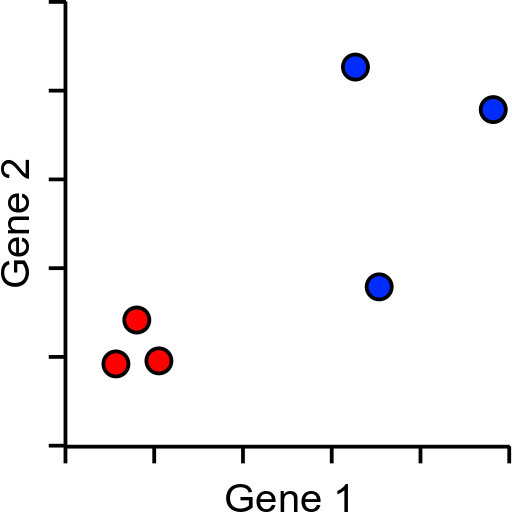
\includegraphics[width=1\textwidth,keepaspectratio]{images/dul/dim-reduce/tsne-points.png}
            \end{figure}
        \end{column}
        \begin{column}{0.33\textwidth}
            \begin{figure}
                \centering
                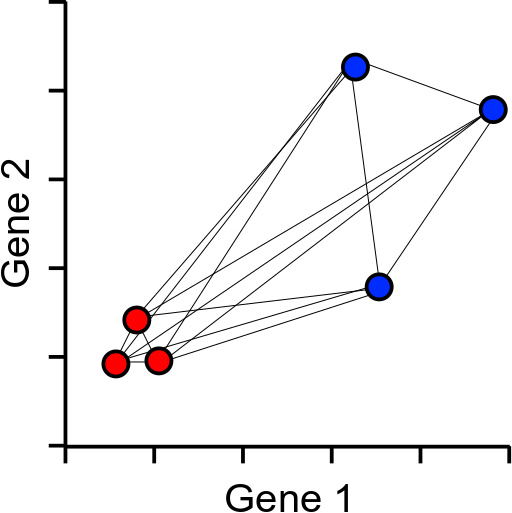
\includegraphics[width=1\textwidth,keepaspectratio]{images/dul/dim-reduce/tsne-graph.png}
            \end{figure}
        \end{column}
        \begin{column}{0.33\textwidth}
            \begin{figure}
                \centering
                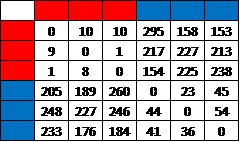
\includegraphics[width=1\textwidth,keepaspectratio]{images/dul/dim-reduce/tsne-matrix.png}
            \end{figure}
        \end{column}
    \end{columns}
\end{frame}

\begin{frame}[allowframebreaks]{tSNE: Underlying idea}
    \begin{figure}
        \centering
        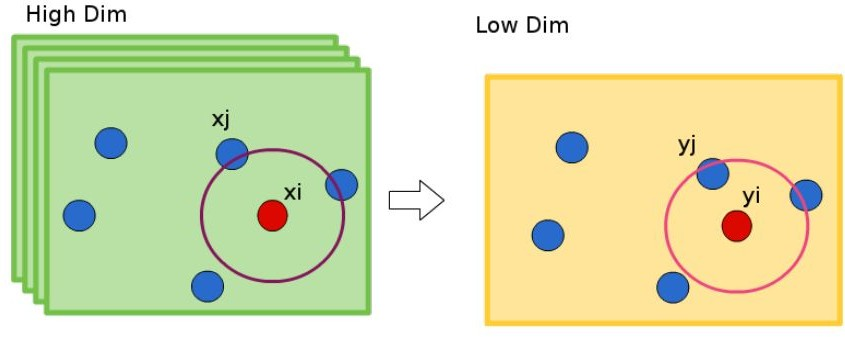
\includegraphics[width=1\textwidth,keepaspectratio]{images/dul/dim-reduce/tsne-high2low.jpg}
    \end{figure}
\end{frame}

\begin{frame}[allowframebreaks]{tSNE: Stochastic Neighbor Embedding}
    \begin{figure}
        \centering
        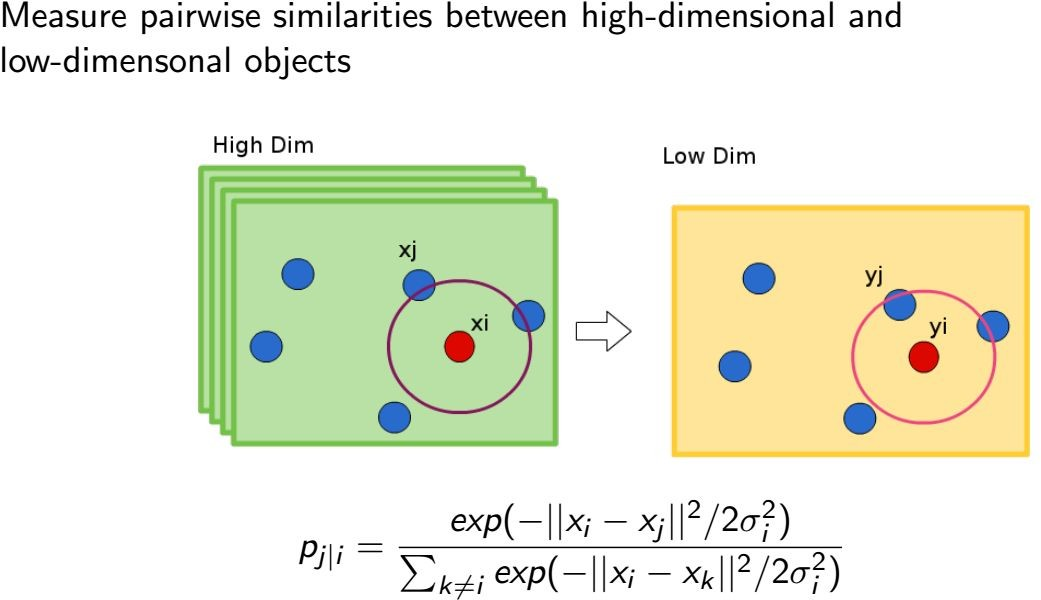
\includegraphics[width=1\textwidth,keepaspectratio]{images/dul/dim-reduce/tsne-stochastic.jpg}
    \end{figure}

    \framebreak

    \begin{figure}
        \centering
        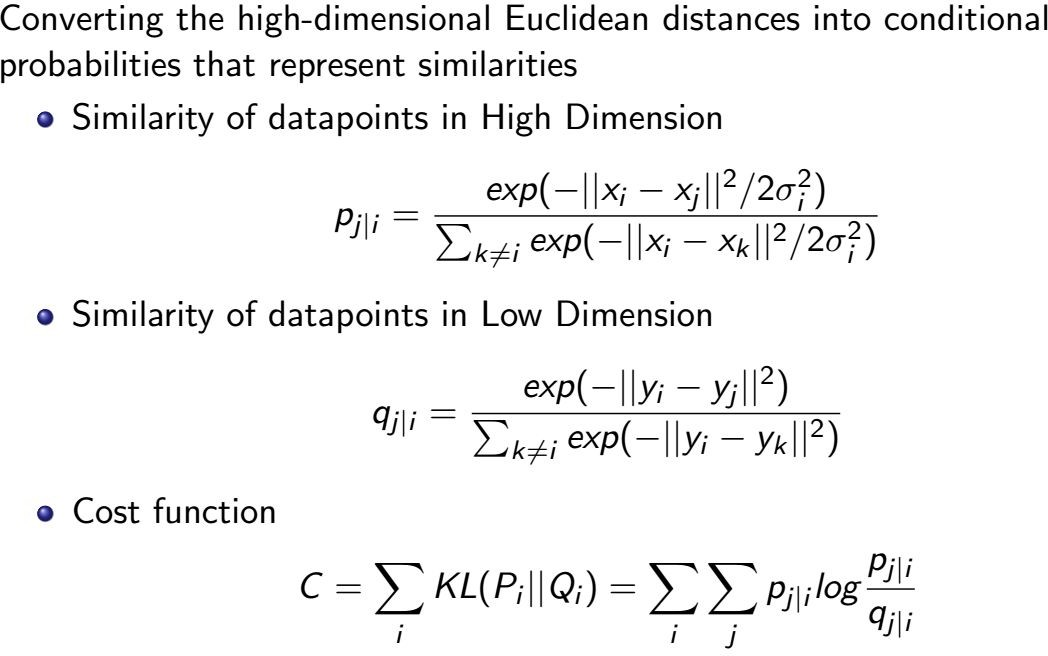
\includegraphics[width=1\textwidth,keepaspectratio]{images/dul/dim-reduce/tsne-stochastic-steps.jpg}
    \end{figure}
\end{frame}

\begin{frame}[allowframebreaks]{KL Divergence}
    \begin{columns}
    \begin{column}{0.4\textwidth}
        Measures the similarity between two probability distributions & it is asymmetric.

        \vspace{1em}

        \begin{figure}
            \centering
            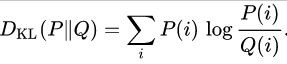
\includegraphics[width=1\textwidth,keepaspectratio]{images/dul/dim-reduce/tsne-similarity.jpg}
        \end{figure}
    \end{column}
    \begin{column}{0.6\textwidth}
        \begin{figure}
            \centering
            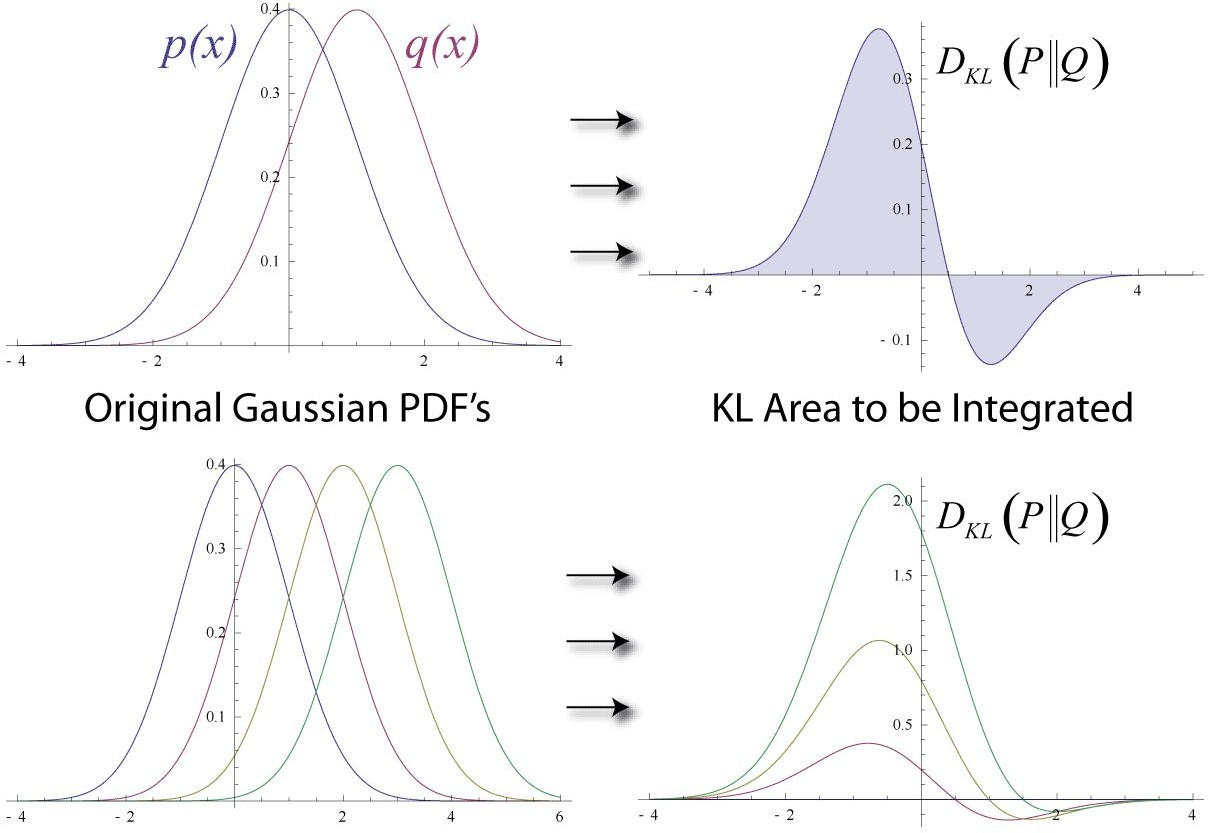
\includegraphics[width=1\textwidth,keepaspectratio]{images/dul/dim-reduce/tsne-similarity-graph.jpg}
        \end{figure}
    \end{column}
    \end{columns}
\end{frame}

\begin{frame}[allowframebreaks]{tSNE: Stochastic Neighbor Embedding}
    \begin{figure}
        \centering
        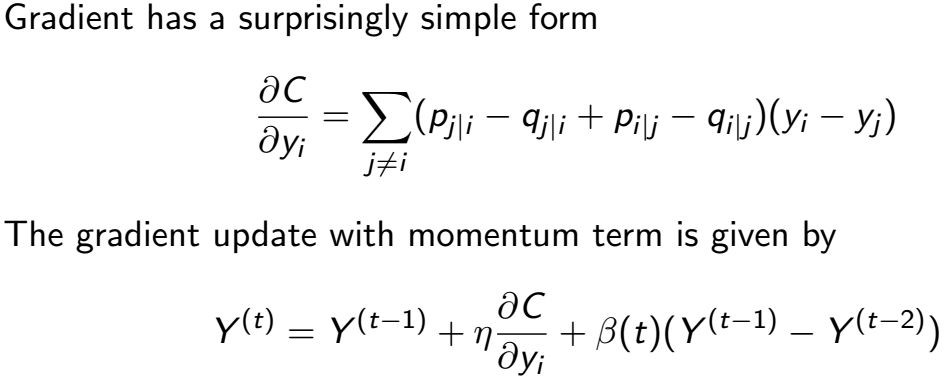
\includegraphics[width=1\textwidth,keepaspectratio]{images/dul/dim-reduce/tsne-gradient.jpg}
    \end{figure}

    \framebreak

    \begin{columns}
    \begin{column}{0.4\textwidth}
        \begin{itemize}
            \item The result of running the SNE algorithm on 3000 256-dimensional grayscale images of handwritten digits.
            \item The classes are quite well separated even though SNE had no information about class labels.
            \item Furthermore, within each class, properties like orientation, skew, and stroke thickness tend to vary smoothly across the space.
        \end{itemize}
    \end{column}
    \begin{column}{0.6\textwidth}
        \begin{figure}
            \centering
            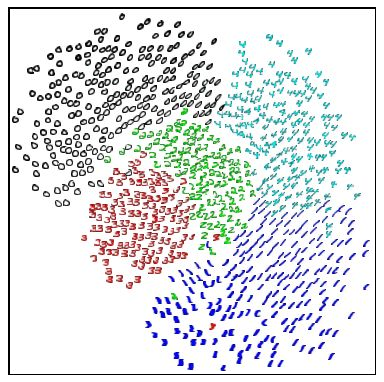
\includegraphics[width=1\textwidth,keepaspectratio]{images/dul/dim-reduce/tsne-result-1.png}
        \end{figure}
    \end{column}
    \end{columns}
\end{frame}

\begin{frame}[allowframebreaks]{Symmetric SNE}
    \begin{figure}
        \centering
        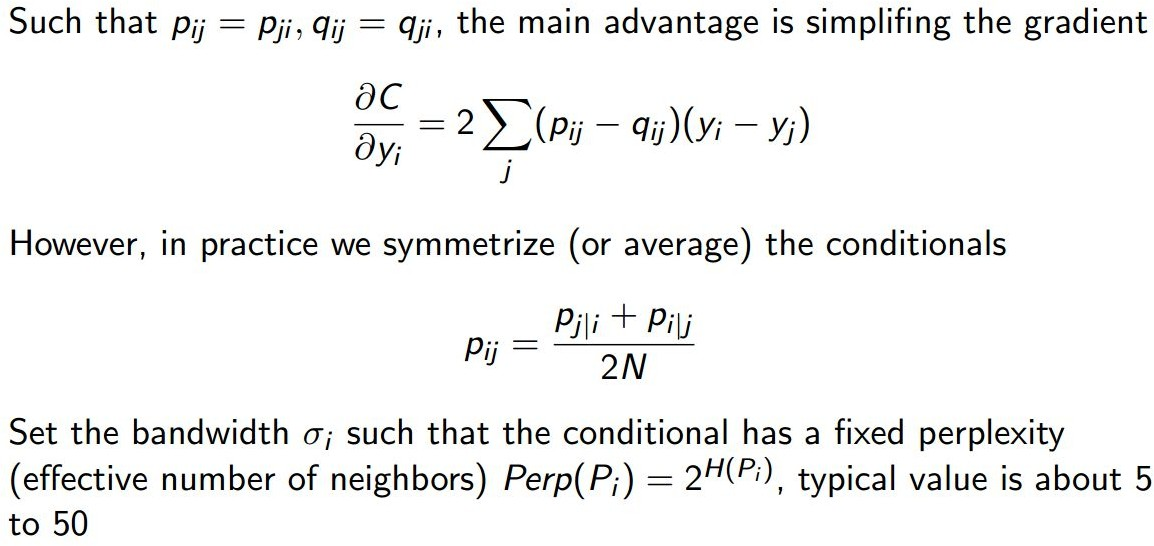
\includegraphics[width=1\textwidth,keepaspectratio]{images/dul/dim-reduce/symmetric-sne.jpg}
    \end{figure}
\end{frame}

\begin{frame}[allowframebreaks]{t-Distribution}
    \begin{figure}
        \centering
        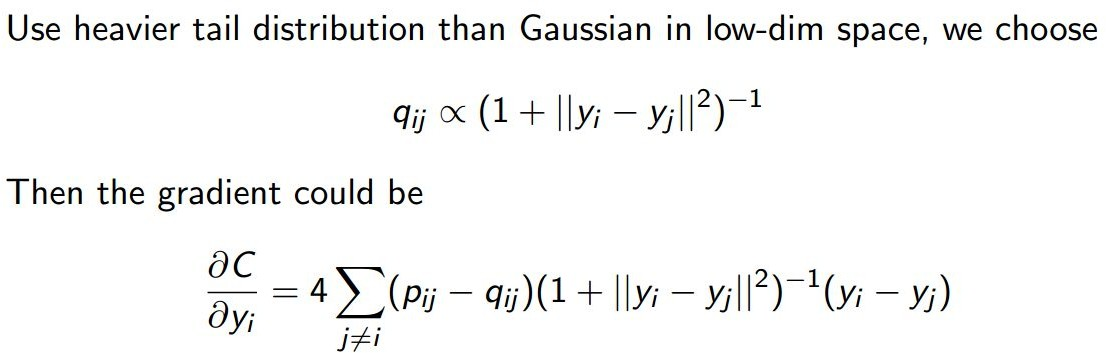
\includegraphics[width=1\textwidth,keepaspectratio]{images/dul/dim-reduce/t-distribution.jpg}
    \end{figure}
\end{frame}

\begin{frame}[allowframebreaks]{Student's t-Distribution}
    \begin{columns}
    \begin{column}{0.5\textwidth}
        \begin{itemize}
            \item Why do we define map similarities as:
            \begin{equation*}
                q_{ij} = \frac{(1 + \|y_i - y_j\|^2)^{-1}}{\sum_{k \neq l} (1 + \|y_k - y_l\|^2)^{-1}}
            \end{equation*}
            \item Suppose data is intrinsically high dimensional
            \item We try to model the local structure of this data in the map
            \item Result: Dissimilar points have to be modeled as too far apart in the map!
        \end{itemize}
    \end{column}
    \begin{column}{0.5\textwidth}
        \begin{figure}
            \centering
            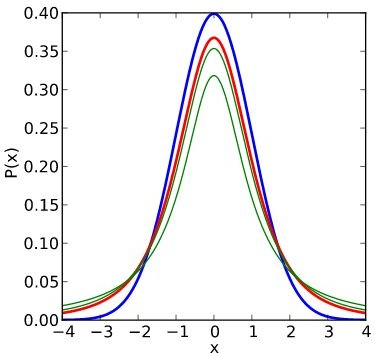
\includegraphics[width=1\textwidth,keepaspectratio]{images/dul/dim-reduce/stundets-t-distrubution.jpg}
        \end{figure}
    \end{column}
    \end{columns}
\end{frame}

\begin{frame}[allowframebreaks]{t-Distributed Stochastic Neighbor Embedding}
    \begin{figure}
        \centering
        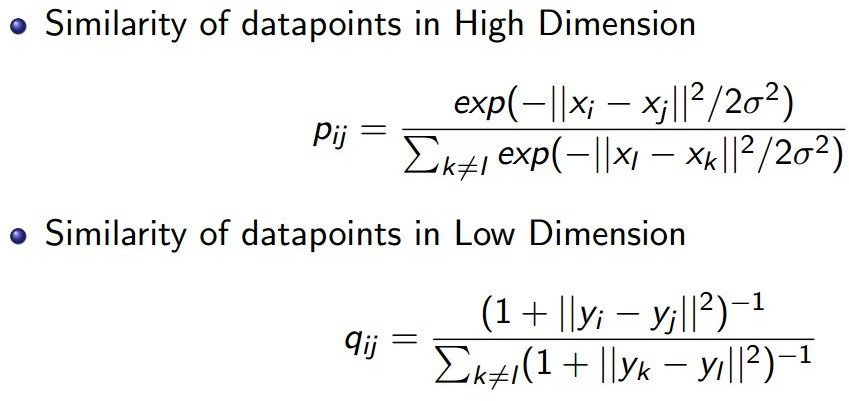
\includegraphics[width=1\textwidth,keepaspectratio]{images/dul/dim-reduce/t-distributed-stochastic.jpg}
    \end{figure}

    \framebreak

    \begin{figure}
        \centering
        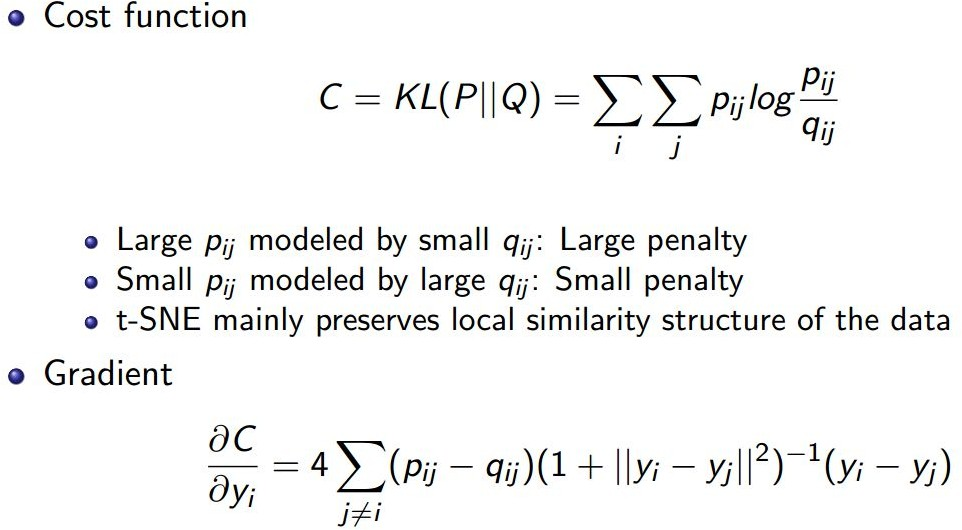
\includegraphics[width=1\textwidth,keepaspectratio]{images/dul/dim-reduce/t-distributed-stochastic-cost.jpg}
    \end{figure}
\end{frame}

\begin{frame}[allowframebreaks]{Distance scaling and perplexity}
    \begin{itemize}
        \item Perplexity = expected number of neighbours within a cluster
        \item Distances scaled relative to perplexity neighbours
    \end{itemize}
    \begin{columns}
    \begin{column}{0.5\textwidth}
        \begin{figure}
            \centering
            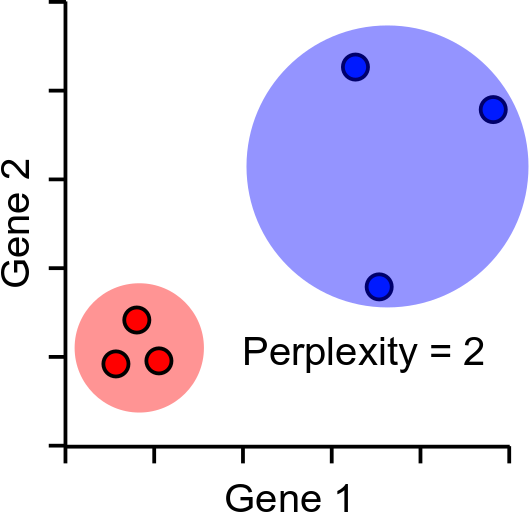
\includegraphics[width=1\textwidth,keepaspectratio]{images/dul/dim-reduce/tsne-distance-scaling.png}
        \end{figure}
    \end{column}
    \begin{column}{0.5\textwidth}
        \begin{figure}
            \centering
            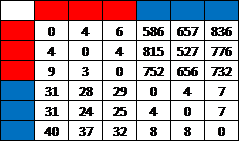
\includegraphics[width=1\textwidth,keepaspectratio]{images/dul/dim-reduce/tsne-distance-scaling-matrix.png}
        \end{figure}
    \end{column}
    \end{columns}
\end{frame}

\begin{frame}[allowframebreaks]{Perplexity Robustness}
    \begin{columns}
    \begin{column}{0.33\textwidth}
        \begin{figure}
            \centering
            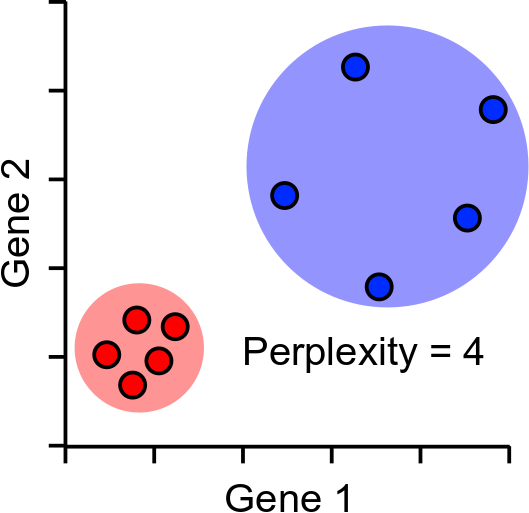
\includegraphics[width=1\textwidth,keepaspectratio]{images/dul/dim-reduce/slide_29_1_img.png}
        \end{figure}
    \end{column}
    \begin{column}{0.33\textwidth}
        \begin{figure}
            \centering
            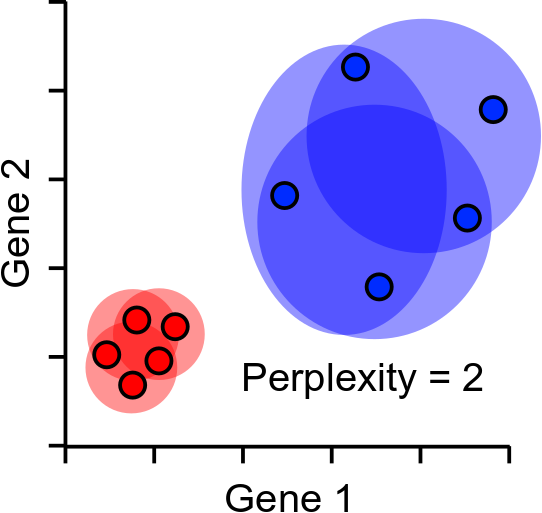
\includegraphics[width=1\textwidth,keepaspectratio]{images/dul/dim-reduce/slide_29_2_img.png}
        \end{figure}
    \end{column}
    \begin{column}{0.33\textwidth}
        \begin{figure}
            \centering
            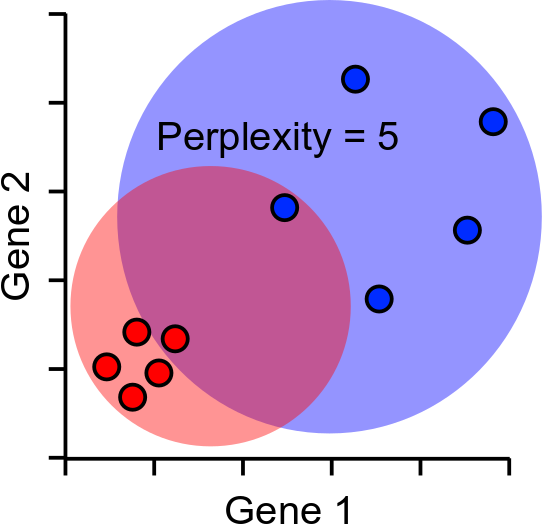
\includegraphics[width=1\textwidth,keepaspectratio]{images/dul/dim-reduce/slide_29_3_img.png}
        \end{figure}
    \end{column}
    \end{columns}
\end{frame}

\begin{frame}[allowframebreaks]{tSNE Projection}
    \begin{itemize}
        \item Randomly scatter all points within the space (normally 2D)
        \item Start a simulation
        \begin{itemize}
            \item Aim is to make the point distances match the distance matrix
            \item Shuffle points based on how well they match
            \item Stop after fixed number of iterations, or
            \item Stop after distances have converged
        \end{itemize}
    \end{itemize}

    \framebreak

    \begin{columns}
    \begin{column}{0.2\textwidth}
        \begin{figure}
            \centering
            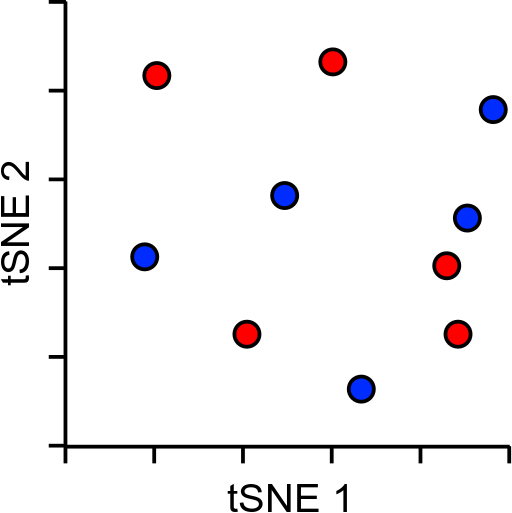
\includegraphics[width=1\textwidth,keepaspectratio]{images/dul/dim-reduce/slide_31_1_img.png}
        \end{figure}
    \end{column}
    \begin{column}{0.2\textwidth}
        \begin{figure}
            \centering
            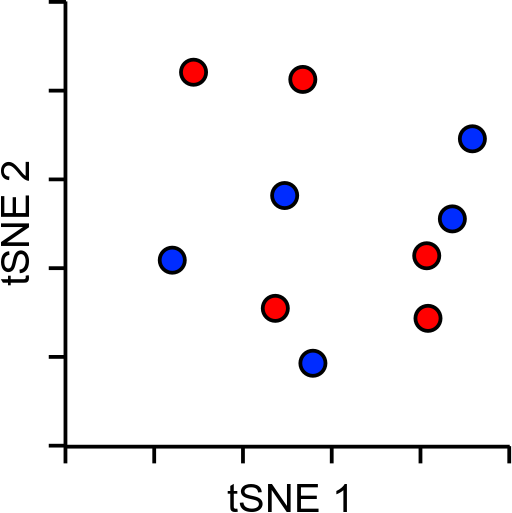
\includegraphics[width=1\textwidth,keepaspectratio]{images/dul/dim-reduce/slide_31_2_img.png}
        \end{figure}
    \end{column}
    \begin{column}{0.2\textwidth}
        \begin{figure}
            \centering
            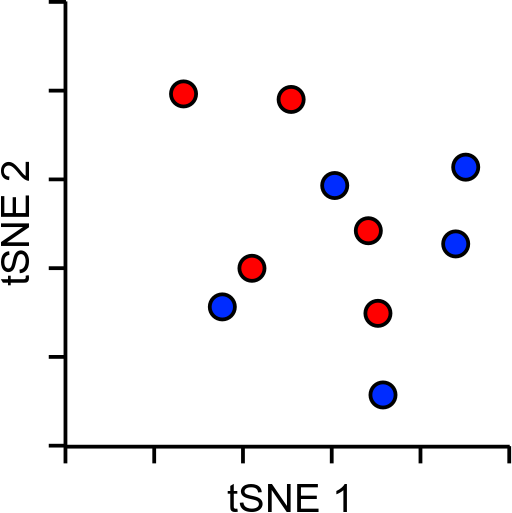
\includegraphics[width=1\textwidth,keepaspectratio]{images/dul/dim-reduce/slide_31_3_img.png}
        \end{figure}
    \end{column}
    \begin{column}{0.2\textwidth}
        \begin{figure}
            \centering
            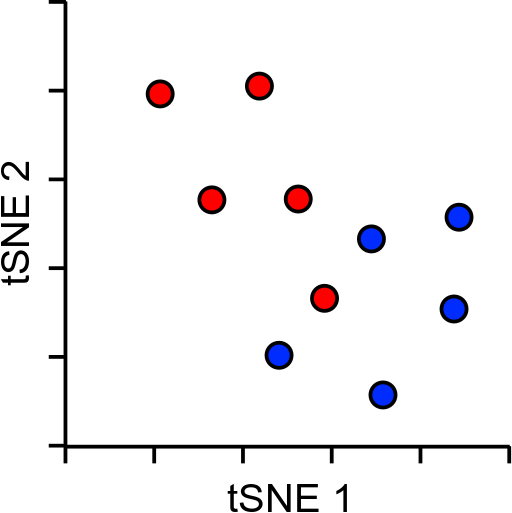
\includegraphics[width=1\textwidth,keepaspectratio]{images/dul/dim-reduce/slide_31_4_img.png}
        \end{figure}
    \end{column}
    \begin{column}{0.2\textwidth}
        \begin{figure}
            \centering
            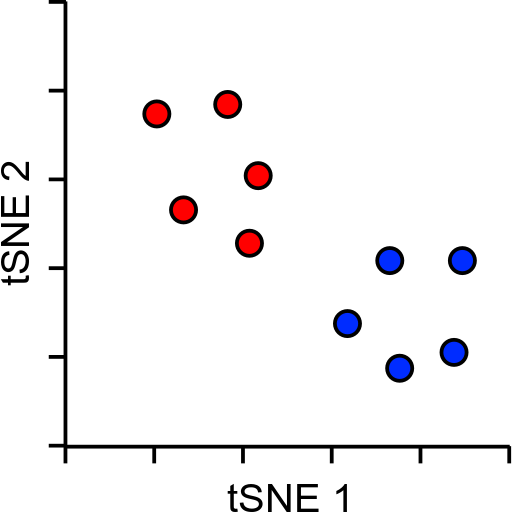
\includegraphics[width=1\textwidth,keepaspectratio]{images/dul/dim-reduce/slide_31_5_img.png}
        \end{figure}
    \end{column}
    \end{columns}

    \vspace{3em}
    \begin{itemize}
        \item X and Y don’t mean anything (unlike PCA)
        \item Distance doesn’t mean anything (unlike PCA)
        \item Close proximity is highly informative
        \item Distant proximity isn’t very interesting
        \item Can’t rationalise distances, or add in more data
    \end{itemize}
\end{frame}

\begin{frame}[allowframebreaks]{tSNE: Practical Examples}
    \begin{figure}
        \centering
        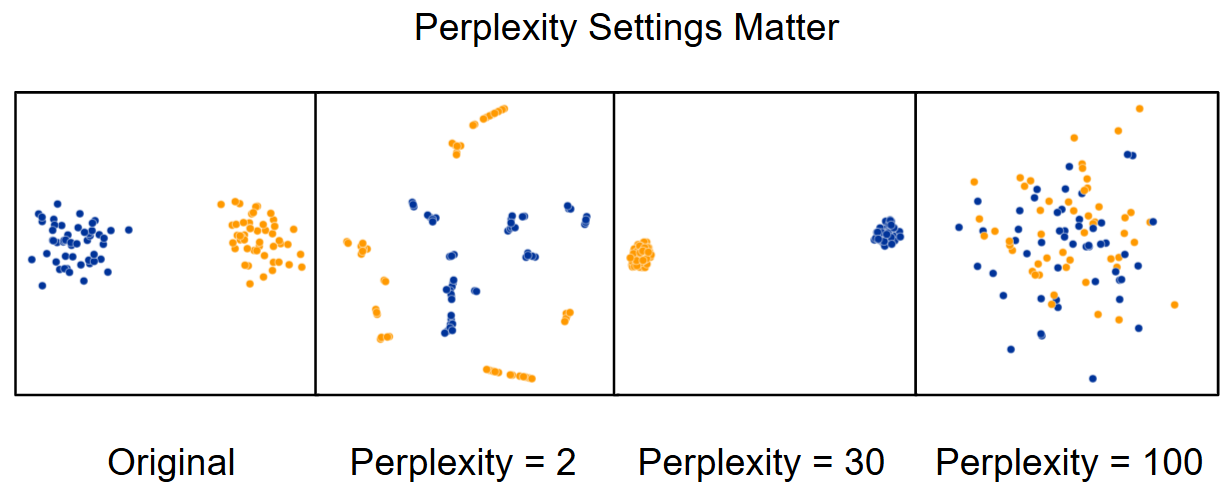
\includegraphics[width=1\textwidth,keepaspectratio]{images/dul/dim-reduce/tsne-perplexity-settings.png}
    \end{figure}

    \framebreak

    \begin{figure}
        \centering
        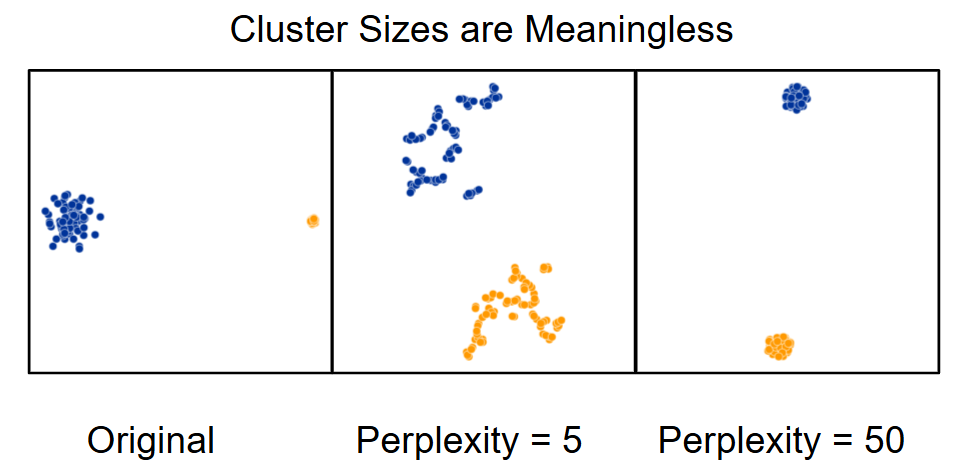
\includegraphics[width=1\textwidth,keepaspectratio]{images/dul/dim-reduce/tsne-perplexity-settings-2.png}
    \end{figure}

    \framebreak

    \begin{figure}
        \centering
        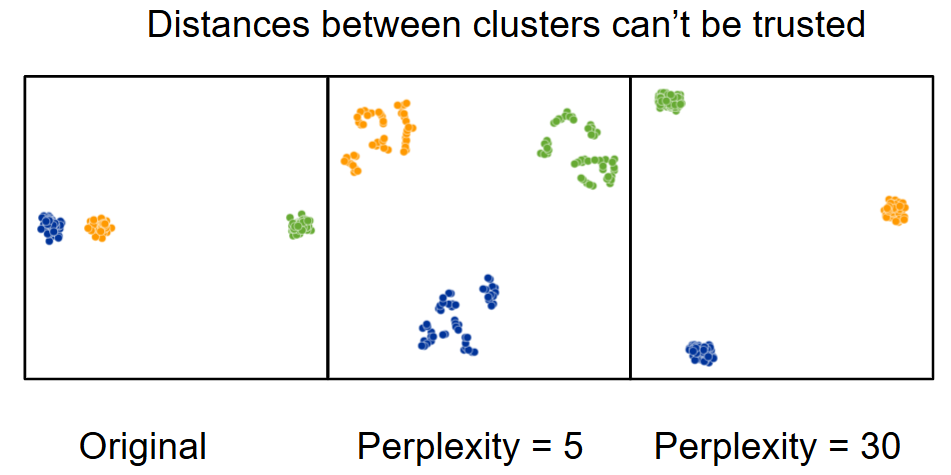
\includegraphics[width=1\textwidth,keepaspectratio]{images/dul/dim-reduce/tsne-perplexity-settings-3.png}
    \end{figure}
\end{frame}

\begin{frame}[allowframebreaks]{tSNE: Results on MNIST}
    \begin{figure}
        \centering
        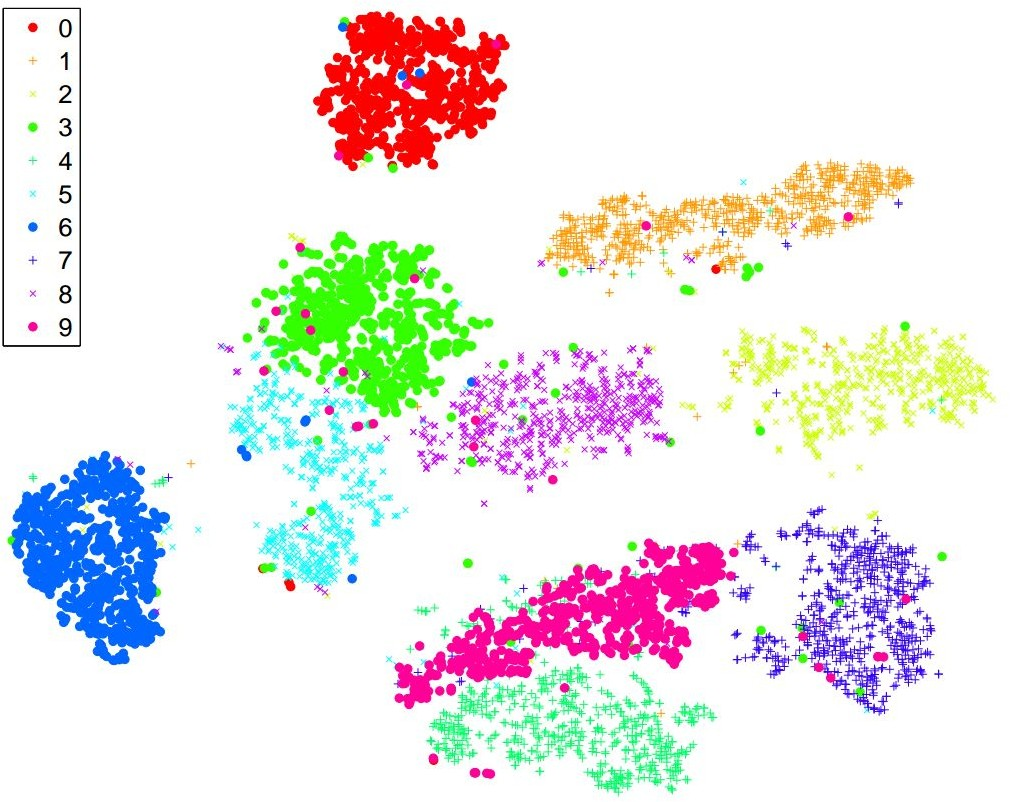
\includegraphics[width=0.9\textwidth,keepaspectratio]{images/dul/dim-reduce/slide_35_1_img.jpg}
    \end{figure}
\end{frame}

\begin{frame}[allowframebreaks]{So tSNE is great then?}
    Kind of\dots

    Imagine a dataset with only one super informative gene

    \begin{columns}
    \begin{column}{0.33\textwidth}
        \begin{figure}
            \centering
            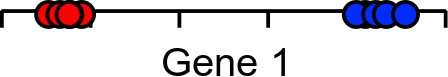
\includegraphics[width=1\textwidth,keepaspectratio]{images/dul/dim-reduce/slide_36_1_img.png}
        \end{figure}

        \vspace{1em}

Distance within cluster = low

\vspace{1em}
        
Distance between clusters = high
    \end{column}
    \begin{column}{0.33\textwidth}
        \begin{figure}
            \centering
            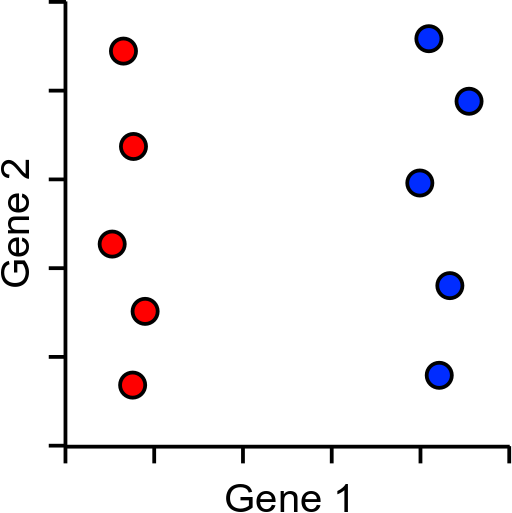
\includegraphics[width=1\textwidth,keepaspectratio]{images/dul/dim-reduce/slide_36_2_img.png}
        \end{figure}
        
        \vspace{1em}

Distance within cluster = higher

\vspace{1em}
        
Distance between clusters = lower
    \end{column}
    \begin{column}{0.33\textwidth}
        \begin{itemize}
            \item First - 3 genes
            \item Second -  3,000 genes
            \item Everything is the same distance from everything
        \end{itemize}
    \end{column}
    \end{columns}
\end{frame}

\begin{frame}[allowframebreaks]{So there is no clear solution?}
    \begin{columns}
    \begin{column}{0.5\textwidth}
        PCA:
        \begin{itemize}
            \item Requires more than 2 dimensions
            \item Expects linear relationships
        \end{itemize}
    \end{column}
    \begin{column}{0.5\textwidth}
        tSNE:
        \begin{itemize}
            \item Can’t cope with noisy data
            \item Loses the ability to cluster
        \end{itemize}
    \end{column}
    \end{columns}

    \framebreak

    \begin{columns}
    \begin{column}{0.5\textwidth}
        PCA:
        \begin{itemize}
            \item Requires more than 2 dimensions
            \item Expects linear relationships
        \end{itemize}
    \end{column}
    \begin{column}{0.5\textwidth}
        tSNE:
        \begin{itemize}
            \item Can’t cope with noisy data
            \item Loses the ability to cluster
        \end{itemize}
    \end{column}
    \end{columns}
    \vspace{1em}
    \textbf{Answer: Combine the two methods, get the best of both worlds!}
    \vspace{1em}
    \begin{columns}
    \begin{column}{0.5\textwidth}
        PCA:
        \begin{itemize}
            \item Good at extracting signal from noise
            \item Extracts informative dimensions
        \end{itemize}
    \end{column}
    \begin{column}{0.5\textwidth}
        tSNE:
        \begin{itemize}
            \item Can reduce to 2D well
            \item Can cope with non-linear scaling
        \end{itemize}
    \end{column}
    \end{columns}
    \vspace{1em}
    \textbf{This is what many pipelines do in their default analysis!}

\end{frame}

\begin{frame}[allowframebreaks]{So PCA + tSNE is great then?}
    Kind of\dots
    \begin{itemize}
        \item tSNE is slow—this is its biggest drawback.
        \begin{itemize}
            \item tSNE does not scale well to large datasets (10,000+ samples).
        \end{itemize}
        \item tSNE provides reliable information only about the closest neighbors; large distance information is mostly irrelevant.
    \end{itemize}
\end{frame}